%%% Sekce - Nástroje pro návrh
%%%%% Wording: ✅
%%%%% Styling: ✅
%%%%% References: ✅
%%%%% Grammar: ✅
%%% --------------------------------------------------------------
\section{Nástroje pro návrh}
\label{sec:navrh-ui-nastroje}
Při navrhování efektivního a efektivního uživatelského rozhraní hraje výběr vhodného návrhového nástroje zásadní roli.
Vybraný nástroj musí mít schopnosti transformovat koncepční nápady a uživatelské příběhy do funkčního designu při dodržení nejlepších postupů a standardů.
Všechny tři široce uznávané nástroje v oblasti návrhu uživatelského rozhraní, jmenovitě \foreign{Adobe XD}, \foreign{Figma} a \foreign{Sketch}, nabízejí jedinečnou sadu funkcí a mají své vlastní silné a slabé stránky\cite{w_how_to_20_best_ui_design_tools}.

Následující části poskytují přehled těchto tří nástrojů s podrobným popisem jejich klíčových funkcí, silných a slabých stránek.
Po srovnávací analýze bude zvolen nástroj pro tento projekt a jeho výběr bude zdůvodněn.
\pagebreak

%%% Podsekce - Adobe XD
%%%%% Wording: ✅
%%%%% Styling: ✅
%%%%% References: ✅
%%%%% Grammar: ✅
%%% --------------------------------------------------------------
\begin{subsection}{Adobe XD}
    \label{subsec:navrh-ui-nastroje-adobe-xd}
    \foreign{Adobe XD (Experience Design)} je vektorový nástroj vyvinutý a publikovaný společností \foreign{Adobe Inc.}
    Primárně se používá pro návrh a prototypování \ac{ux} pro webové a mobilní aplikace.
    Adobe XD usnadňuje celý proces návrhu od nápadu a návrhu po prototypování a náhled \ac{ux}~\cite{adobe-xd}.

    \begin{figure}[H]
        \centering
        \caption{Logo nástroje Adobe XD}
        
\includegraphics[width=0.8\textwidth]{\FIGDIR/adobe-xd-logo}
        \source[\citeauthor{adobe-xd}]{}
        \label{fig:adobe-xd-logo}
    \end{figure}

    Adobe XD, jehož logo je zobrazeno na obrázku~\ref{fig:adobe-xd-logo}, je součástí \foreign{Adobe Creative Cloud}, který se integruje s dalšími nástroji \foreign{Adobe}, jako je \foreign{Photoshop} a \foreign{Illustrator}, a nabízí bezproblémovou kompatibilitu souborů.
    Mezi jeho klíčové funkčnosti patří:
    \begin{itemize}
        \item \textbf{Repeat Grid}: Tato funkce umožňuje návrhářům replikovat designové prvky, což šetří čas při návrhu složitých \ac{ui}.
        \item \textbf{Prototypování a animace}: Adobe XD poskytuje funkce pro vytváření interaktivních prototypů s lehkostí.
        \item \textbf{Voice Prototyping}: Adobe XD poskytuje prototypování hlasu, které lze použít pro návrh hlasových asistentů a dalších hlasem ovládaných aplikací.
        \item \textbf{Kolaborace}: Adobe XD podporuje kolaboraci v reálném čase, což umožňuje více členů týmu pracovat na stejném návrhu současně.
        \item \textbf{Integrace}: Adobe XD se integruje s dalšími nástroji v sadě \foreign{Adobe Creative Cloud} a také s pluginy třetích stran, což poskytuje širokou škálu dalších funkcí.
    \end{itemize}

    \pagebreak
    Na obrázku~\ref{fig:adobe-xd-example} je zobrazena ukázka rozhraní Adobe XD.\
    \begin{figure}[H]
        \centering
        \caption{Ukázka rozhraní nástroje Adobe XD}
        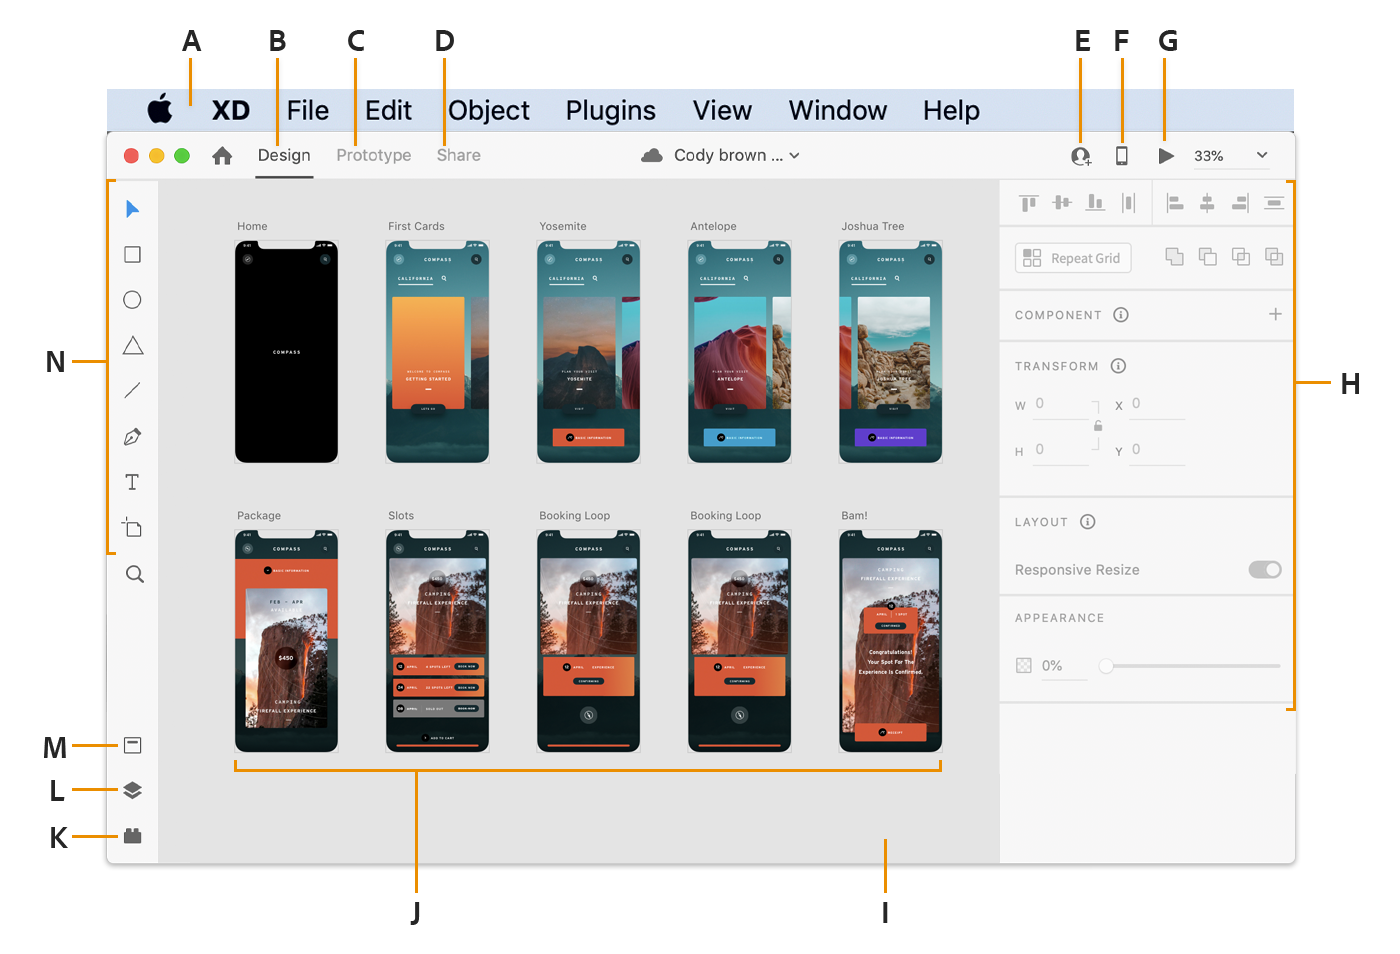
\includegraphics[width=0.8\textwidth]{\FIGDIR/adobe-xd-example}
        \source[\citeauthor{adobe-xd}]{}
        \label{fig:adobe-xd-example}
    \end{figure}

    \textbf{Silné stránky:}
    \begin{itemize}
        \item Bezproblémová integrace s dalšími nástroji \foreign{Adobe}.
        \item Výkonné možnosti prototypování a animace.
        \item Schopnost navrhovat pro různé platformy včetně webu, mobilu, tabletu a dalších.
        \item Silná podpora komunity a zdrojů pro učení.
    \end{itemize}

    \textbf{Slabé stránky:}
    \begin{itemize}
        \item Omezená podpora pro složité animace ve srovnání s některými jinými nástroji.
        \item Je vyžadováno předplatné služby \foreign{Adobe Creative Cloud}, což může být pro některé uživatele drahé.
        \item Možnosti kolaborace jsou dobré, ale mohou být omezenější než v některých jiných nástrojích\cite{w_industry_the_ultimate_battle_figma_vs_sketch_vs_adobe_xd, adobe-xd}.
    \end{itemize}
\end{subsection}

%%% Podsekce - Figma
%%%%% Wording: ✅
%%%%% Styling: ✅
%%%%% References: ✅
%%%%% Grammar: ✅
%%% --------------------------------------------------------------
\begin{subsection}{Figma}
    \label{subsec:navrh-ui-nastroje-figma}
    \foreign{Figma} je webový nástroj pro návrh \ac{ui} a prototypování.
    Získal významnou popularitu díky své pokročilé funkčnosti kolaborace a jeho webové založenosti, která umožňuje spolupráci v reálném čase, což jej činí oblíbeným nástrojem pro mnoho týmů\cite{w_industry_the_ultimate_battle_figma_vs_sketch_vs_adobe_xd}.
    Na obrázku~\ref{fig:figma-logo} je zobrazeno logo nástroje Figma a na obrázku~\ref{fig:figma-example} níže je zobrazena ukázka jeho rozhraní.

    \begin{figure}[H]
        \centering
        \caption{Logo nástroje Figma}
        
\includegraphics[width=0.8\textwidth]{\FIGDIR/figma-logo}
        \source[\citeauthor{figma}]{}
        \label{fig:figma-logo}
    \end{figure}

    Figma umožňuje, aby celý proces návrhu probíhal v rámci nástroje: od \foreign{brainstormingu}\footnote{\foreign{Brainstorming} je technika, která se používá k vytváření velkého množství nápadů na řešení problému.} po vytváření interaktivních prototypů.
    Mezi některé klíčové funkce tohoto nástroje patří:

    \begin{itemize}
        \item \textbf{Kolaborace v reálném čase}: Více lidí může současně pracovat na návrhu, podobně jako v \foreign{Google Docs}, což z Figma činí skvělý nástroj pro týmové projekty.
        \item \textbf{Komponenty a style}: Figma podporuje komponenty (opakovaně použitelné designové prvky) a styly, které podporují konzistenci napříč návrhy a šetří čas.
        \item \textbf{Prototypování a animace}: Figma umožňuje vytvářet interaktivní prototypy s přechody.
        Ačkoli nemusí být tak robustní jako některé jiné nástroje, slouží pro většinu návrhových potřeb.
        \item \textbf{Auto-layout}: Tato funkce umožňuje návrhářům vytvářet responzivní rozložení s lehkostí, což výrazně zrychluje proces návrhu.
    \end{itemize}

    \begin{figure}[H]
        \centering
        \caption{Ukázka rozhraní nástroje Figma}
        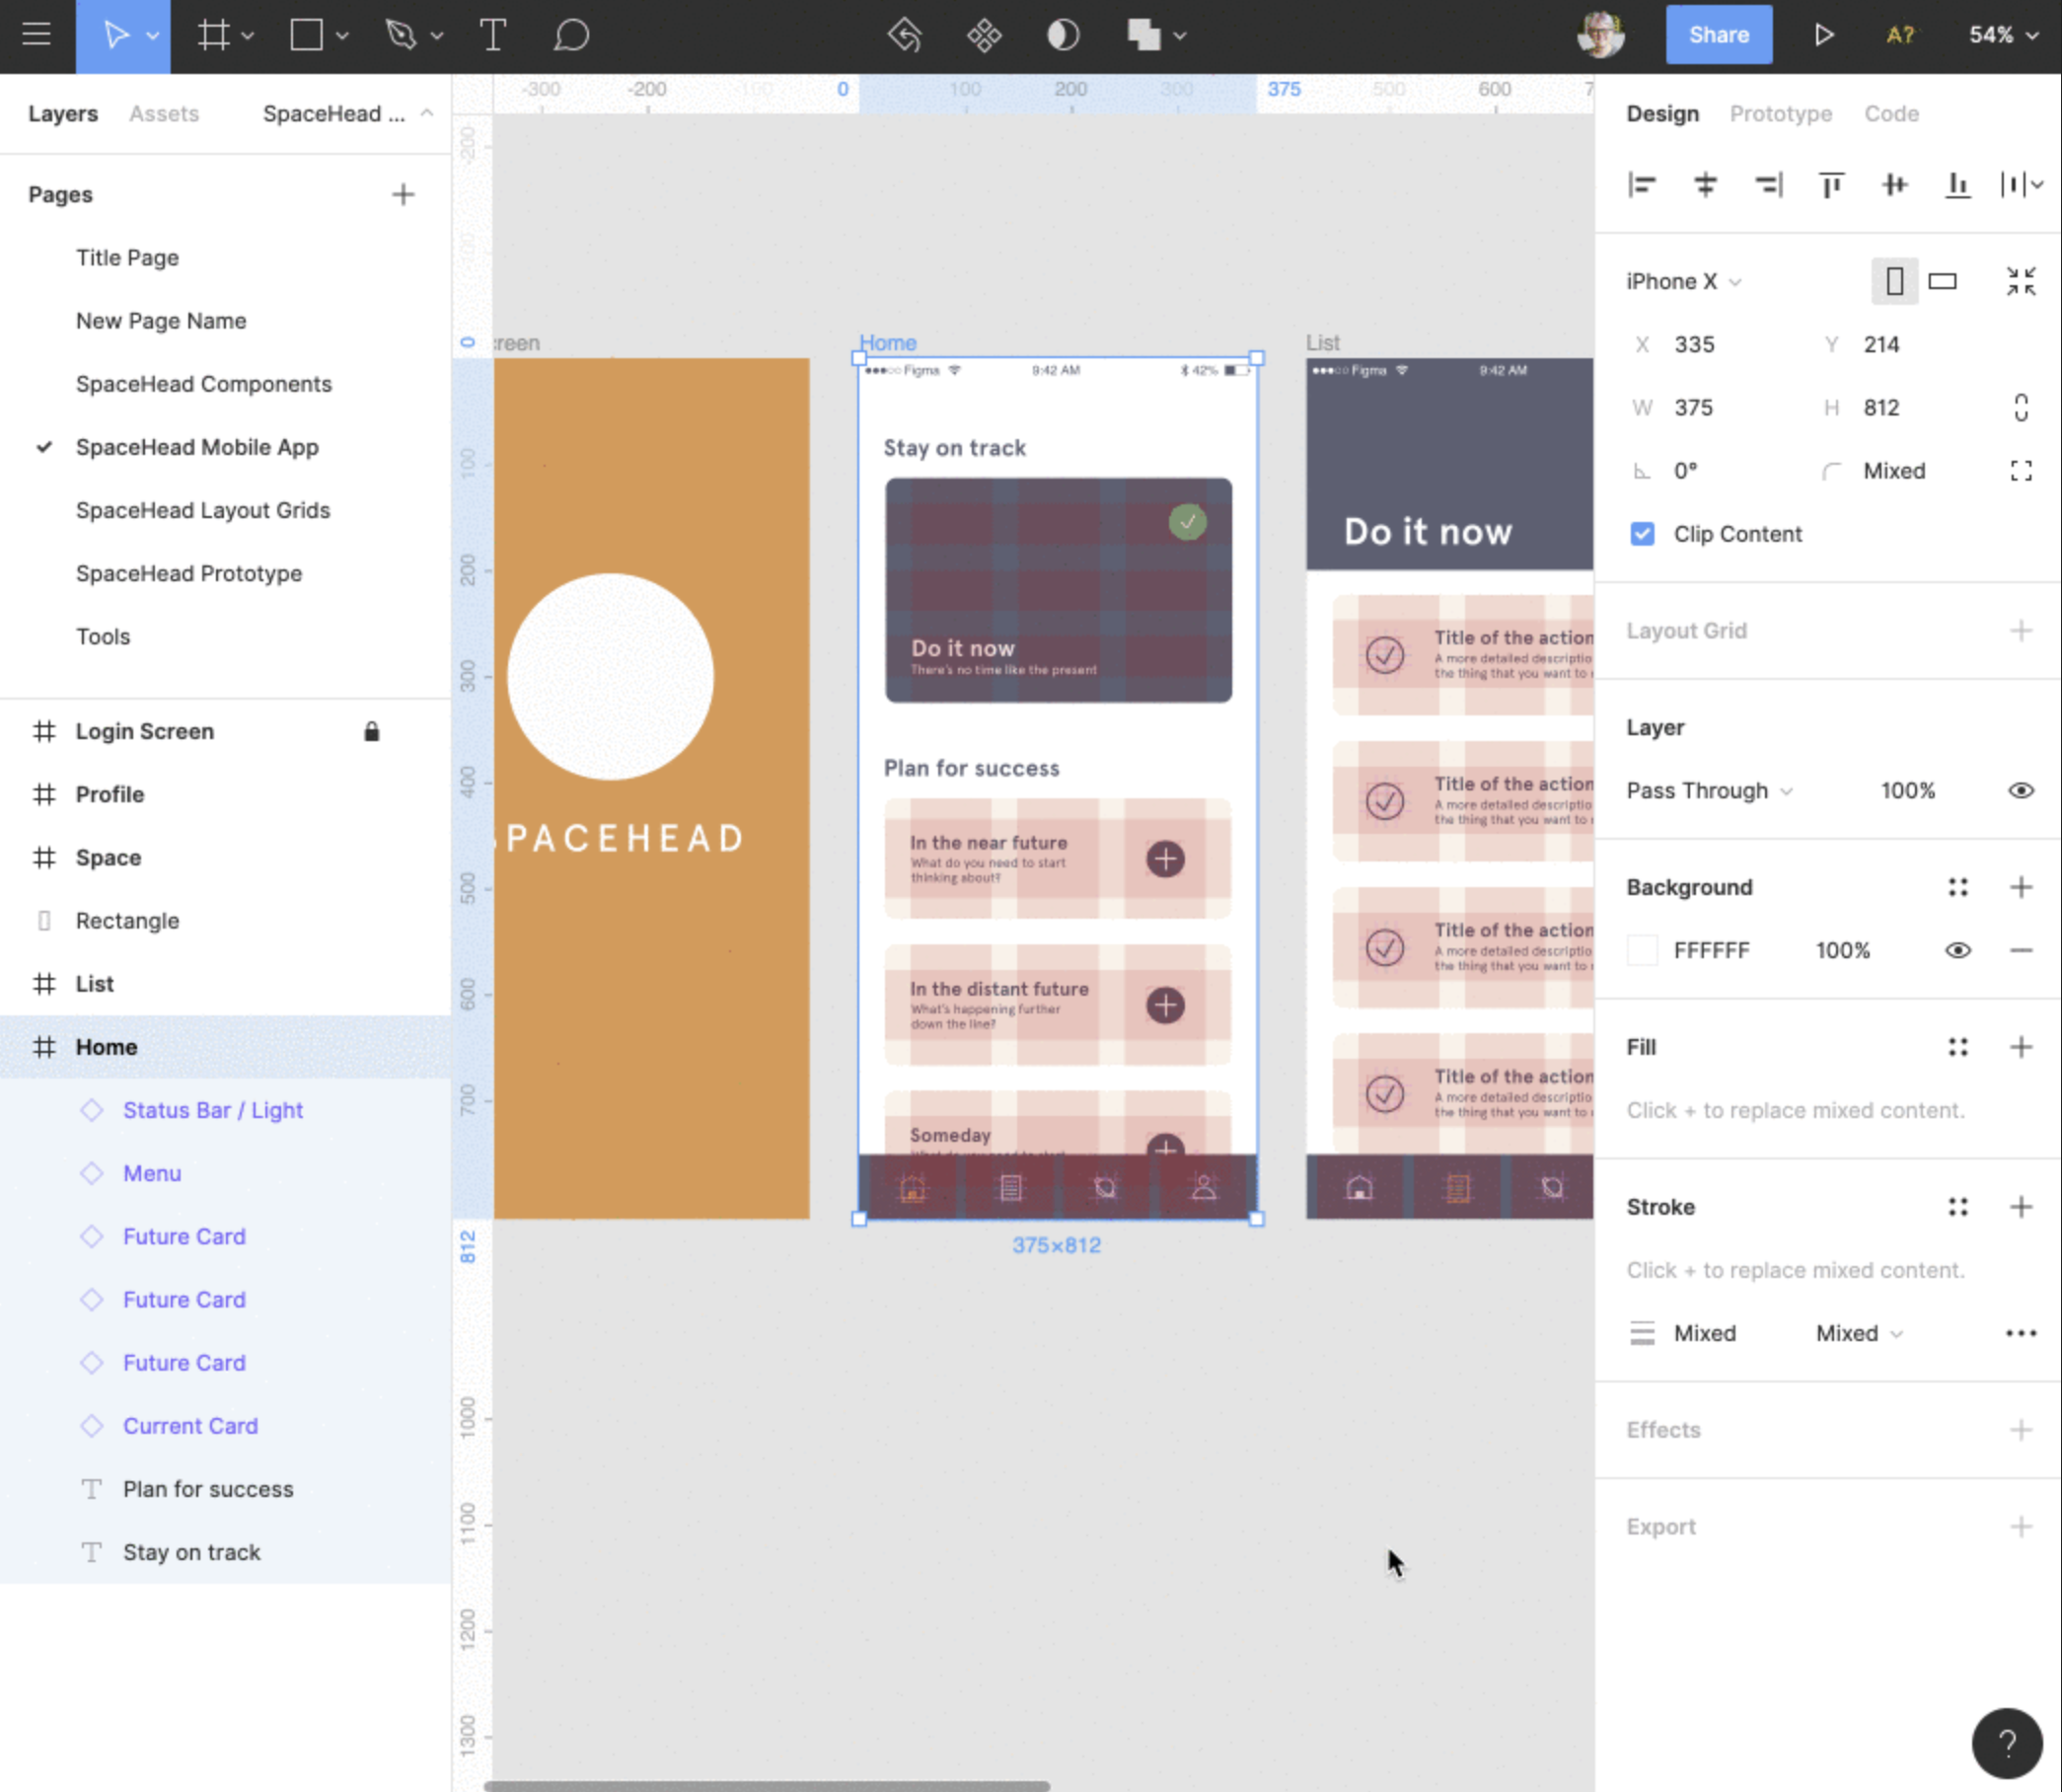
\includegraphics[width=0.8\textwidth]{\FIGDIR/figma-example}
        \source[\citeauthor{figma}]{}
        \label{fig:figma-example}
    \end{figure}

    \textbf{Silné stránky:}
    \begin{itemize}
        \item Umožňuje spolupráci a společné úpravy v reálném čase.
        \item Není třeba stahovat software; veškerá práce je uložena a přístupná prostřednictvím cloudu.
        \item Zahrnuje design, prototypování a předávací nástroje na jednom místě.
        \item Nezávislé na platformě, funguje v prohlížeči.
    \end{itemize}

    \textbf{Slabé stránky:}
    \begin{itemize}
        \item Omezené možnosti práce v offline režimu
        \item Pro většinu funkcí je vyžadováno připojení k internetu.
        \item Na méně výkonných počítačích může běžet pomaleji\cite{w_industry_the_ultimate_battle_figma_vs_sketch_vs_adobe_xd, h_hc_en_us}.
    \end{itemize}
\end{subsection}

%%% Podsekce - Sketch
%%%%% Wording: ✅
%%%%% Styling: ✅
%%%%% References: ✅
%%%%% Grammar: ✅
%%% --------------------------------------------------------------
\begin{subsection}{Sketch}
    \label{subsec:navrh-ui-nastroje-sketch}
    \foreign{Sketch}, jenž byl kdysi průmyslovým standardem pro návrh \ac{ui} a \ac{ux}, je vektorový nástroj pro návrh \ac{ui} a \ac{ux} pro macOS\@.
    Byl spuštěn v roce 2010 a od té doby získal významnou uživatelskou základnu\cite{w_industry_the_ultimate_battle_figma_vs_sketch_vs_adobe_xd}.
    Logo tohoto nástroje je zobrazeno na obrázku~\ref{fig:sketch-logo} a ukázka jeho rozhraní je zobrazena na obrázku~\ref{fig:sketch-example} níže.

    \begin{figure}[H]
        \centering
        \caption{Logo nástroje Sketch}
        
\includegraphics[width=0.8\textwidth]{\FIGDIR/sketch-logo}
        \source[\citeauthor{sketch}]{}
        \label{fig:sketch-logo}
    \end{figure}

    Sketch je primárně určen pro návrh rozhraní a prototypování.
    Některé z jeho klíčových funkcí jsou:

    \begin{itemize}
        \item \textbf{Symboly a styly}: Sketch podporuje symboly (opakovaně použitelné designové prvky) a styly, které podporují konzistenci napříč návrhy a šetří čas.
        \item \textbf{Pluginy}: Jednou z hlavních sil nástroje Sketch je jeho široká škála pluginů, které lze použít k rozšíření jeho funkcionality.
        \item \textbf{Prototypování}: Zatímco Sketch byl původně za jinými nástroji v oblasti prototypování, v této oblasti učinil významné pokroky.
        \item \textbf{Sdílené knihovny}: Sketch má silnou podporu pro sdílené knihovny, což umožňuje snadné sdílení zdrojů, komponent a stylů napříč projekty.
    \end{itemize}

    \begin{figure}[H]
        \centering
        \caption{Ukázka rozhraní nástroje Sketch}
        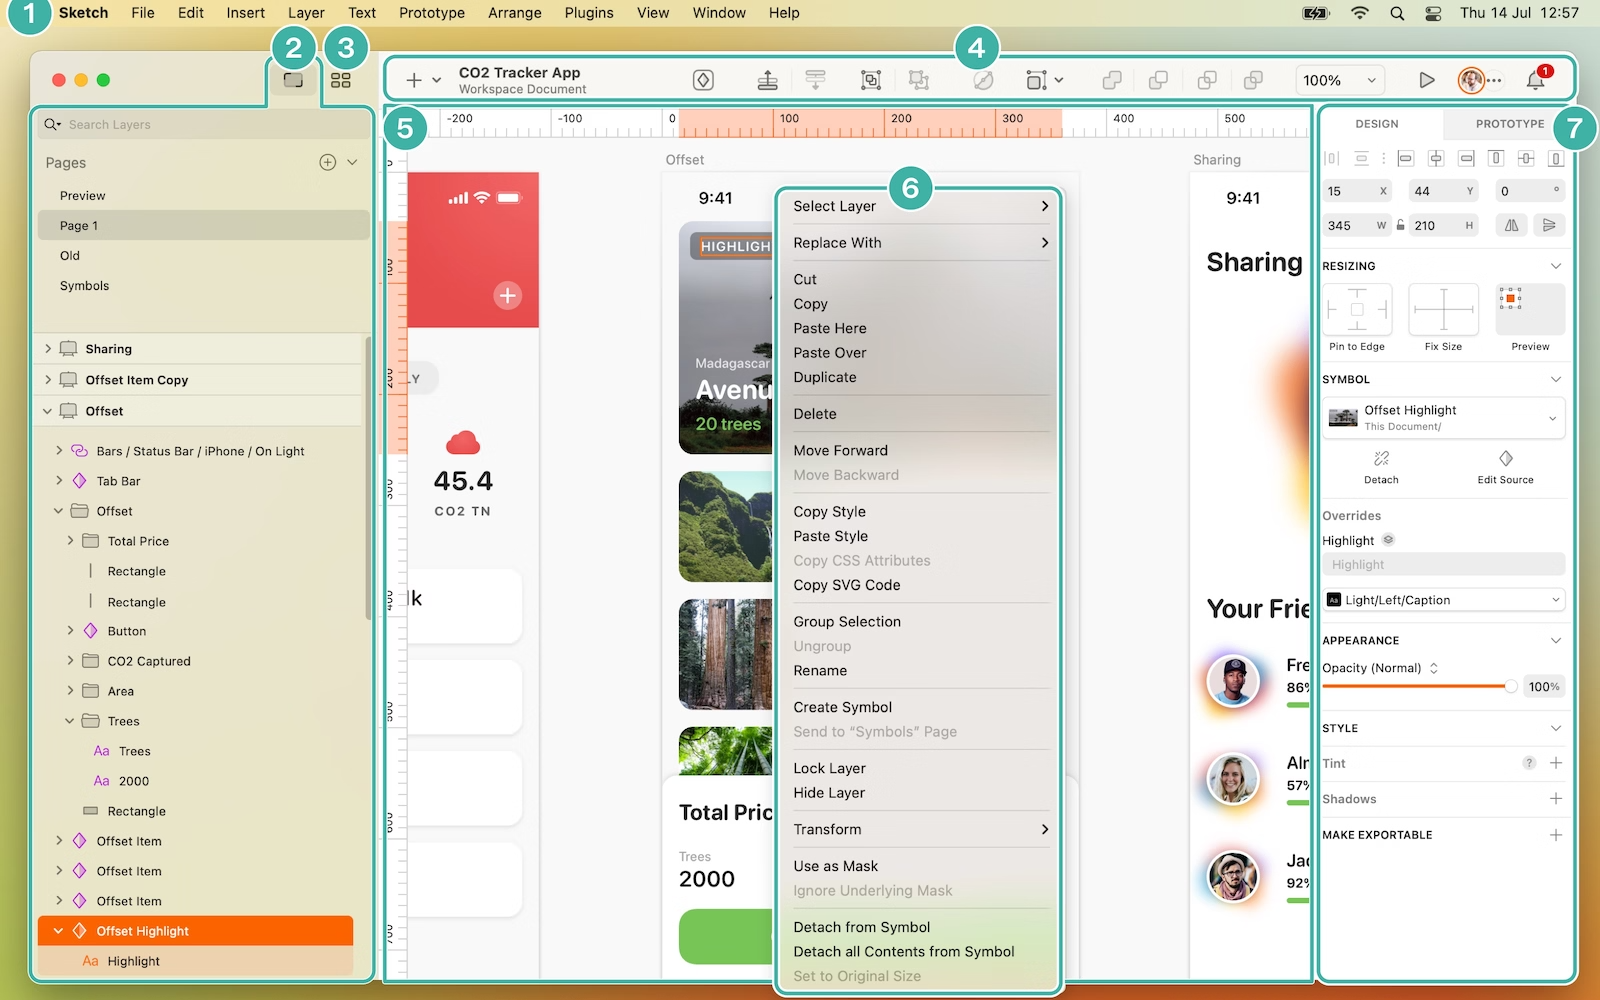
\includegraphics[width=0.8\textwidth]{\FIGDIR/sketch-example}
        \source[\citeauthor{sketch}]{}
        \label{fig:sketch-example}
    \end{figure}

    \textbf{Silné stránky:}
    \begin{itemize}
        \item Široká škála rozšíření/pluginů.
        \item Silná komunita a dostupnost zdrojů.
    \end{itemize}

    \textbf{Slabé stránky:}
    \begin{itemize}
        \item Dostupný pouze pro macOS, což omezuje jeho dostupnost.
        \item Bez vestavěné podpory pro spolupráci nebo společné úpravy\cite{w_industry_the_ultimate_battle_figma_vs_sketch_vs_adobe_xd, sketch}.
    \end{itemize}
\end{subsection}

%%% Podsekce - Výběr nástroje
%%%%% Wording: ✅
%%%%% Styling: ✅
%%%%% References: ✅
%%%%% Grammar: ✅
%%% --------------------------------------------------------------
\begin{subsection}{Výběr nástroje}
    \label{subsec:navrh-ui-nastroje-vyber}
    Aby bylo možné učinit rozhodnutí a vybrat nejvhodnější nástroj pro návrh uživatelského rozhraní pro tento projekt, je nezbytné provést srovnávací analýzu tří nástrojů, které jsou podrobně popsány výše – Adobe XD, Figma a Sketch.
    Nástroje jsou porovnávány v několika klíčových aspektech, včetně platformové a cenové dostupnosti, prototypovacích schopnostech, správy komponent, stylování a knihoven, podpory pluginů, komunity a dostupných zdrojů.

    \pagebreak
    \textbf{Platformová dostupnost}\\
    Figma a Adobe XD vynikají svou dostupností napříč platformami.
    Oba nástroje lze používat na Windows a macOS a Figma je dostupná i na Linuxu, případně jiných OS, prostřednictvím webového prohlížeče.
    Sketch je však omezen pouze na macOS, což může způsobit problémy s kompatibilitou a možnou spoluprací.

    \textbf{Cenová dostupnost}\\
    Adobe XD nabízí bezplatný startovací plán, přičemž placené plány nabízejí více funkcí.
    Figma také nabízí bezplatný plán s dalšími funkcemi dostupnými v profesionálních a týmových plánech.
    Sketch poskytuje bezplatnou zkušební verzi s jednorázovou platbou za plnou verzi a dodatečnými náklady na roční aktualizace.

    \textbf{Prototypování}\\
    Adobe XD, Figma i Sketch nabízejí možnosti prototypování.
    Adobe XD a Figma však poskytují podporu pro složitější a interaktivnější prototypy ve srovnání s aplikací Sketch, která má základní možnosti vytváření prototypů.

    \textbf{Komponenty}\\
    Adobe XD, Figma i Sketch nabízejí knihovny komponent pro zjednodušení procesu navrhování.
    Komponenty a styly Figma jsou pokročilejší, což umožňuje lepší organizaci a efektivitu.

    \textbf{Stylování a knihovny}\\
    Figma a Sketch mají silnou podporu pro sdílené styly a knihovny, které umožňují konzistenci v designu.
    Adobe XD také podporuje sdílené prostředky, ale jeho možnosti nejsou tak robustní jako u nástrojů Figma a Sketch.

    \textbf{Pluginy}\\
    Sketch původně vedl v podpoře pluginů, ale Adobe XD a Figma jej rychle dohnali a všechny tři nástroje nabízejí širokou škálu pluginů pro rozšíření funkčnosti.

    \textbf{Komunita a zdroje}\\
    Sketch je nejstarší z těchto tří nástrojů a má největší komunitu a nejširší škálu zdrojů.
    Nicméně Figma, přestože se jedná o relativně nový nástroj, si díky své popularitě a širokému použití vybudoval silnou komunitu.
    Adobe XD má také podpůrnou komunitu, ale není tak rozsáhlá jako u nástrojů Figma nebo Sketch.

    Stručně řečeno, všechny tři nástroje mají své vlastní silné stránky a uspokojují různé potřeby a preference.
    Toto celé srovnání je souhrnně zobrazeno v tabulce~\ref{tab:ui-design-tools-comparison}.

    \begin{table}[h]
        \centering
        \caption{Srovnání nástrojů pro návrh uživatelského rozhraní}
        \label{tab:ui-design-tools-comparison}
        \resizebox{\textwidth}{!}
        {
        %
            \begin{tabular}{llll}
                \toprule
                \textbf{Funkčnost} & \textbf{Adobe XD} & \textbf{Figma}  & \textbf{Sketch}  \\
                \midrule
                Podpora Windows    & Ano               & Ano             & Ne               \\
                Podpora macOS      & Ano               & Ano             & Ano              \\
                Webová aplikace    & Ne                & Ano             & Ne               \\
                Dostupné zdarma    & Ano               & Ano             & Trial verze      \\
                Placené plány      & od \$9.99/měs.\    & od \$12/měs.\    & \$99/jednorázově \\
                Prototypování      & Ano               & Ano             & Ano              \\
                Komponenty         & Ano               & Ano (pokročilé) & Ano              \\
                Stylování/knihovny & Ano               & Ano (pokročilé) & Ano              \\
                Pluginy            & Ano               & Ano             & Ano              \\
                Komunita a zdroje  & Dobrá             & Výborná         & Výborná          \\
                \bottomrule
            \end{tabular}
        %
        }
        \source{}
    \end{table}

    Po rozboru této analýzy byl vybrán jako preferovaný nástroj pro návrh uživatelského rozhraní zkoumané aplikace nástroj \textbf{Figma}.
    Tato volba byla motivována kombinací několika přesvědčivých faktorů, včetně:

    \begin{enumerate}
        \item \textbf{Dostupnost a podpora platformy}: Figma je platformně nezávislý nástroj a podporuje různé operační systémy, včetně Windows, macOS, a dokonce i Linuxu prostřednictvím webového prohlížeče.
        Tato široká dostupnost je významnou výhodou oproti Sketch, který je dostupný pouze pro macOS\@.
        \item \textbf{Cena}: Figma poskytuje robustní bezplatnou verzi, která umožňuje až tři aktivní projekty.
        Pro tento projekt jsou funkce poskytované v bezplatné verzi dostatečné, což z Figma činí ekonomicky výhodnou volbu.
        \item \textbf{Pokročilý systém komponent}: Systém komponent nástroje Figma je pokročilý a umožňuje hierarchickou organizaci komponent.
        To zajišťuje konzistenci v designu a zjednodušuje proces, zejména při práci s komplexními designy, jako je interaktivní mapa sedadel.
        \item \textbf{Schopnosti prototypování}: Figma značně vyniká, pokud jde o prototypování – umožňuje vytvářet interaktivní prototypy pomocí řady funkcí a přechodů.
        \item \textbf{Komunita a zdroje}: Figma se pyšní rozsáhlou online komunitou a množstvím zdrojů, zajišťuje, že řešení potenciálních problémů během návrhového procesu jsou snadno řešitelné.
        \item \textbf{Osobní zkušenost}: Používaje různé nástroje pro návrh, volba nástroje Figma byla také motivována osobní zkušeností s tímto nástrojem.
    \end{enumerate}

    Tento nástroj kombinuje silnou sadu funkcí s osobní preferencí pro jeho rozhraní a funkčnost, což z něj činí ideální volbu pro tento projekt.

    Nyní je již možné přejít ke konkrétnímu návrhu uživatelského rozhraní rozborem jednotlivých uživatelských příběhů definovaných v předchozí sekci~\ref{sec:navrh-uzivatelskeho-rozhrani-uzivatelske-pribehy}.
\end{subsection}
